\documentclass{article}

\usepackage{graphicx}
\usepackage{amsfonts}
\usepackage{pdfpages}
\usepackage{bbm}
\usepackage{amssymb}
\usepackage[margin=1in]{geometry}

\title{ STAT 321: Assignment 4}
\author{Saksham Sudershan}
\date{12 March 2022}

\begin{document}
	\maketitle
	\section*{Problem 1}
	Let $D=1$ be the event that the rater is diligent and $D=0$ be the event that the rater is non-diligant. Let $S_i=1$ be the event that $i$ number of content are labeled as spam, and $S_i=0$ be the event that $i$ number of content are labeled as non-spam. Now,
	$$ P(D=1)=0.90\ and\ P(D=0)=0.10 $$
	$$ P(S_1=1|D=1)=0.20\ and\ P(S_1=0|D=1)=0.80 $$
	$$ P(S_1=1|D=0)=0\ and\ P(S_1=1|D=0)=1 $$

	Now, using Bayes Theorem,
	$$ P(D=1|S_4=0)=\frac{P(S_4=0|D=1)\cdot P(D=1)}{P(S_4=0|D=1)\cdot P(D=1)+P(S_4=0|D=0)\cdot P(D=1)} $$


	We also know that,
	$$ P(S_4=1|D=1)=0.8^4\ and\ P(S_4=1|D=0)=1^4$$

	$$ \therefore P(D=1|S_4=0) = \frac{0.8^4 \cdot 0.90}{0.8^4 \cdot 0.90+1^4 \cdot 0.10}$$
	$$ \Rightarrow P(D=1|S_4=0) \approx 0.7866 $$

	\section*{Problem 2}
	Let $Y$ be the number of friends that say it is raining in Vancouver. And let $R$ be the event that it is raining in Vancouver.
	$$ P(R) = 0.25 \ and\ P(R') = 0.75$$
	
	Using Bayes Theorem,
	$$ P(R|Y=3) = \frac{P(Y=3|R) \cdot P(R)}{P(Y=3|R) \cdot P(R) + P(Y=3|R') \cdot P(R')}$$

	Now, the probability that each of the friend is lying is $\frac13$. So,
	$$ P(Y=3|R) = \left( \frac{2}{3}\right)^3 \ and\ P(Y=3|R') = \left( \frac{1}{3} \right)^3$$

	Putting this together, we get,
	$$ P(R|Y=3) = \frac{\left( \frac{2}{3} \right)^3 \cdot0.25}{\left( \frac{2}{3} \right)^3 \cdot0.25 + \left( \frac{1}{3} \right)^3 \cdot 0.75} $$
	$$ \Rightarrow P(R|Y=3) \approx 0.7273 $$

	\section*{Problem 3}
		\subsection*{(a)}
			Let $E$ be the event that we win, that is, $\mathbb{HH}$ shows up first.  Let $H_i$ and $T_i$ be the event that $\mathbb{H}$ or $\mathbb{T}$ show up for the $i$th toss. Now,

			$$ P(E|H_1) = \frac{1}{2}$$
			$$ P(H_1) = \frac{1}{2}$$

			$$ And\ P(E|T_1) = 0 $$
			$$ P(T) = \frac{1}{2} $$

			Using Law of Total Probability,
			$$ P(E) = P(E|H_1) \cdot P(H_1) + P(E|T_1) \cdot P( T_1) $$
			$$ \Rightarrow P(E) = 0.50 \cdot 0.50 + 0 \cdot 0.50 = 0.25 $$
			So the probability of us winning is $0.25$. 

		\subsection*{(b)}
			In this case, let $E$ be the event that our friends wins, that is, $\mathbb{HHT}$ shows up first.  Let $H_i$ and $T_i$ be the event that $\mathbb{H}$ or $\mathbb{T}$ show up for the $i$th toss. Now, 

			$$Let\ P(E)=p$$
			$$ Then\ P(E|T_1)=p $$
			$$ Let\ P(E|H_1) = q $$

			Using the Law of Total Probability,
			$$ P(E) = P(E|H_1) \cdot P(H_1) + P(E|T_1) \cdot P( T_1)  $$
			$$ \Rightarrow p = p \cdot \frac{1}{2} + q \cdot \frac{1}{2} $$
			$$ \Rightarrow p = q $$

			Now, considering the first two rolls,
			$$ P(E| H_1 \cap H_2 ) = 1 $$
			$$ P(E| H_1 \cap T_2 ) = \frac{1}{2} \times p $$
			$$ P(E| T_1 \cap H_2 ) = q = p  $$
			$$ and P(E| T_1 \cap T_2 ) = p $$

			$$ We\ know\ that\ P(H_1 \cap H_2 ) = 0.25 \, , P(T_1 \cap H_2 ) = 0.25, $$
			$$  \ P(H_1 \cap T_2 ) = 0.25 \ and\ P(T_1 \cap T_2 )=0.25$$

			Again, using the Law of Total Probability,
			$$ P(E) =  P(E| H_1 \cap H_2 )\cdot 0.25 +  P(E| H_1 \cap T_2 )\cdot 0.25 +  P(E| T_1 \cap H_2 )\cdot 0.25 + P(E| T_1 \cap T_2 )\cdot 0.25 $$

			$$ \therefore p = 0.25 \times \left[ 1 + 0.5 \cdot p + p +p \right] $$
			$$ \Rightarrow p = 0.25\times [2.5p + 1] $$
			$$ \Rightarrow 4p - 2.5p = 1 $$
			$$ \Rightarrow 1.5p = 1 $$
			$$ \Rightarrow p \approx 0.667 $$

			$$ \therefore P(Our\ friend\ winning) = 0.667 $$
			$$ \Rightarrow P(Us\ winning) = 1 - p = 0.333 $$
			So the probability of us winning is $0.333$. 

	\section*{Problem 4}
		\subsection*{(a)}
		$Y$ is the random variable which denotes the number of balls in bin 1. There are a total of $n$ number of balls. Thus, we can say that $Y\sim Binom(y,p)$, where $p=1/10$.
		So the pmf of Y is given by,
		$$ p_Y(y) = {n \choose y} \left( \frac{1}{10} \right)^y \left( \frac{9}{10} \right)^{n-y} \; \; \; \; \; \; \; where\ 0\leq y \leq n $$

		\subsection*{(b)}
		$Z$ is the random variable which denotes the number of balls in bin 6,7,8,9 and 10. There are a total of $n$ number of balls. Thus, we can say that $Z\sim Binom(z,p)$, where $p=5/10$.
		So the pmf of Z is given by,
		$$ p_Z(z) = {n \choose z} \left( \frac{5}{10} \right)^z \left( \frac{5}{10} \right)^{n-z} \; \; \; \; \; \; \; where\ 0\leq z \leq n $$

		\subsection*{(c)}
		Given that there are $y$ number of balls in bin 1, there are $n-y$ balls left. We also know that from $n-y$ balls, none go into bin 1. So,
		$$ p_{Z|Y}(z|y) = {n-y \choose z} \left( \frac{5}{9} \right)^z \left( \frac{4}{9} \right)^{n-y-z}  \; \; \; \; \; \; \; where\ 0\leq y \leq n \ and\ 0 \leq z \leq n-y $$

		\subsection*{(d)}
		Given that there are $z$ number of balls in bins 6-10, there are $n-z$ balls left. We also know that from $n-z$ balls, none go into bin 6-10. So,
		$$ p_{Y|Z}(y|z) = {n-z \choose y} \left( \frac{1}{5} \right)^y \left( \frac{4}{5} \right)^{n-z-y}  \; \; \; \; \; \; \; where\ 0\leq z \leq n \ and\ 0 \leq y \leq n-z $$

	\section*{Problem 5}
	Let $R_i$ and $B_i$ represent that the $i$th ball pulled out is red and blue respectively.
		\subsection*{(a)}
			$$ P(R_1) = \frac{1}{2} $$
		\subsection*{(b)}
			$$ P(R_2) = P(R_2|R_1) \cdot P(R_1) + P(R_2|B_1) \cdot P(B_1) $$
			$$ \Rightarrow P(R_2) = \frac{2}{3} \cdot \frac{1}{2} + \frac{1}{3} \cdot \frac{1}{2} $$
			$$ \Rightarrow P(R_2) = \frac{1}{2} $$
		\subsection*{(c)}
			$$ P(R_3 \cap R_2 \cap R_1) = P(R_3|R_2 \cap R_1) \cdot P(R_2|R_1) \cdot P(R_1) $$
			$$ \Rightarrow P(R_3 \cap R_2 \cap R_1) = \frac{3}{4} \cdot \frac{2}{3} \cdot {1}{2} $$
			$$ \Rightarrow P(R_3 \cap R_2 \cap R_1) = \frac{1}{4} $$
		\subsection*{(d)}
			$$ P(2\ of\ the\ first\ 3\ balls\ are\ red) = P(R_1 \cap R_2 \cap B_3) + P(R_1 \cap B_2 \cap R_3) + P(B_1 \cap R_2 \cap R_3) $$
			$$ \Rightarrow P(2\ of\ 3\ are\ red) = \left( \frac{1}{2} \times \frac{2}{3} \times \frac{1}{4} \right) + \left( \frac{1}{2}\times \frac{1}{3}\times \frac{2}{4}\right) + \left( \frac{1}{2}\times \frac{1}{3}\times \frac{2}{4} \right)$$
			$$ \Rightarrow P(2\ of\ 3\ are\ red) = \frac{1}{12}+\frac{1}{12}+\frac{1}{12} = \frac{1}{4} $$ 

	\section*{Problem 6}
		Using Bayes Theorem,
		$$ f_{P|X}(p|9)= \frac{P(P=p) \cdot P(X=9|P=p)}{P(X=9)}$$
		
		We know that $P\sim$ Unif[0,1], so
		$$ P(P=p) = \frac{1}{1-0} = 1 \; \; \; \; \ \;\ \; \; \;  where 0 \leq p \leq 1 $$

		And we also know that $X\sim$ Binom(10,$P$), so
		$$ P(X=9|P=p) = {10 \choose 9} p^9 (1-p) $$

		Now, $P(P=p)=1$ when $p \in [0,1]$. So we can integrate $P(X=9|P=p)$ for all $p \in [0,1]$ to find $P(X=9)$. So,
		$$ P(X=9) = \int_{0}^{1} {10 \choose 9} p^9 (1-p) $$
		$$ \Rightarrow P(X=9)= {10 \choose 9} \int_{0}^{1} p^9-p^{10} $$
		$$ \Rightarrow P(X=9)= {10 \choose 9} \left[ \frac{p^{10}}{10} - \frac{p^{11}}{11}\right]_{0}^{1} $$
		$$ \Rightarrow P(X=9)= {10 \choose 9}  \left[ \frac{1}{10} - \frac{1}{11}\right] $$
		$$ \Rightarrow P(X=9)= {10 \choose 9} \cdot \frac{1}{110} $$

		Putting this all together,
		$$  f_{P|X}(p|9)= \frac{ {10 \choose 9} p^9 (1-p) }{ {10 \choose 9} \cdot \frac{1}{110} }$$
		$$ \Rightarrow   f_{P|X}(p|9)= 110 \cdot p^9 (1-p) $$


		Sketching this, 

		\centering
		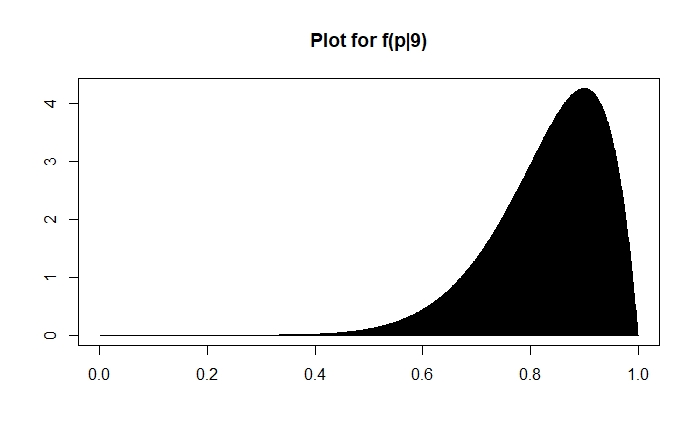
\includegraphics[width=\textwidth]{Rplot}
\end{document}